\documentclass[tikz,border=5pt]{standalone}
\usepackage{tikz}
\usepackage{booktabs}
\usetikzlibrary{automata, positioning, arrows.meta}
\begin{document}
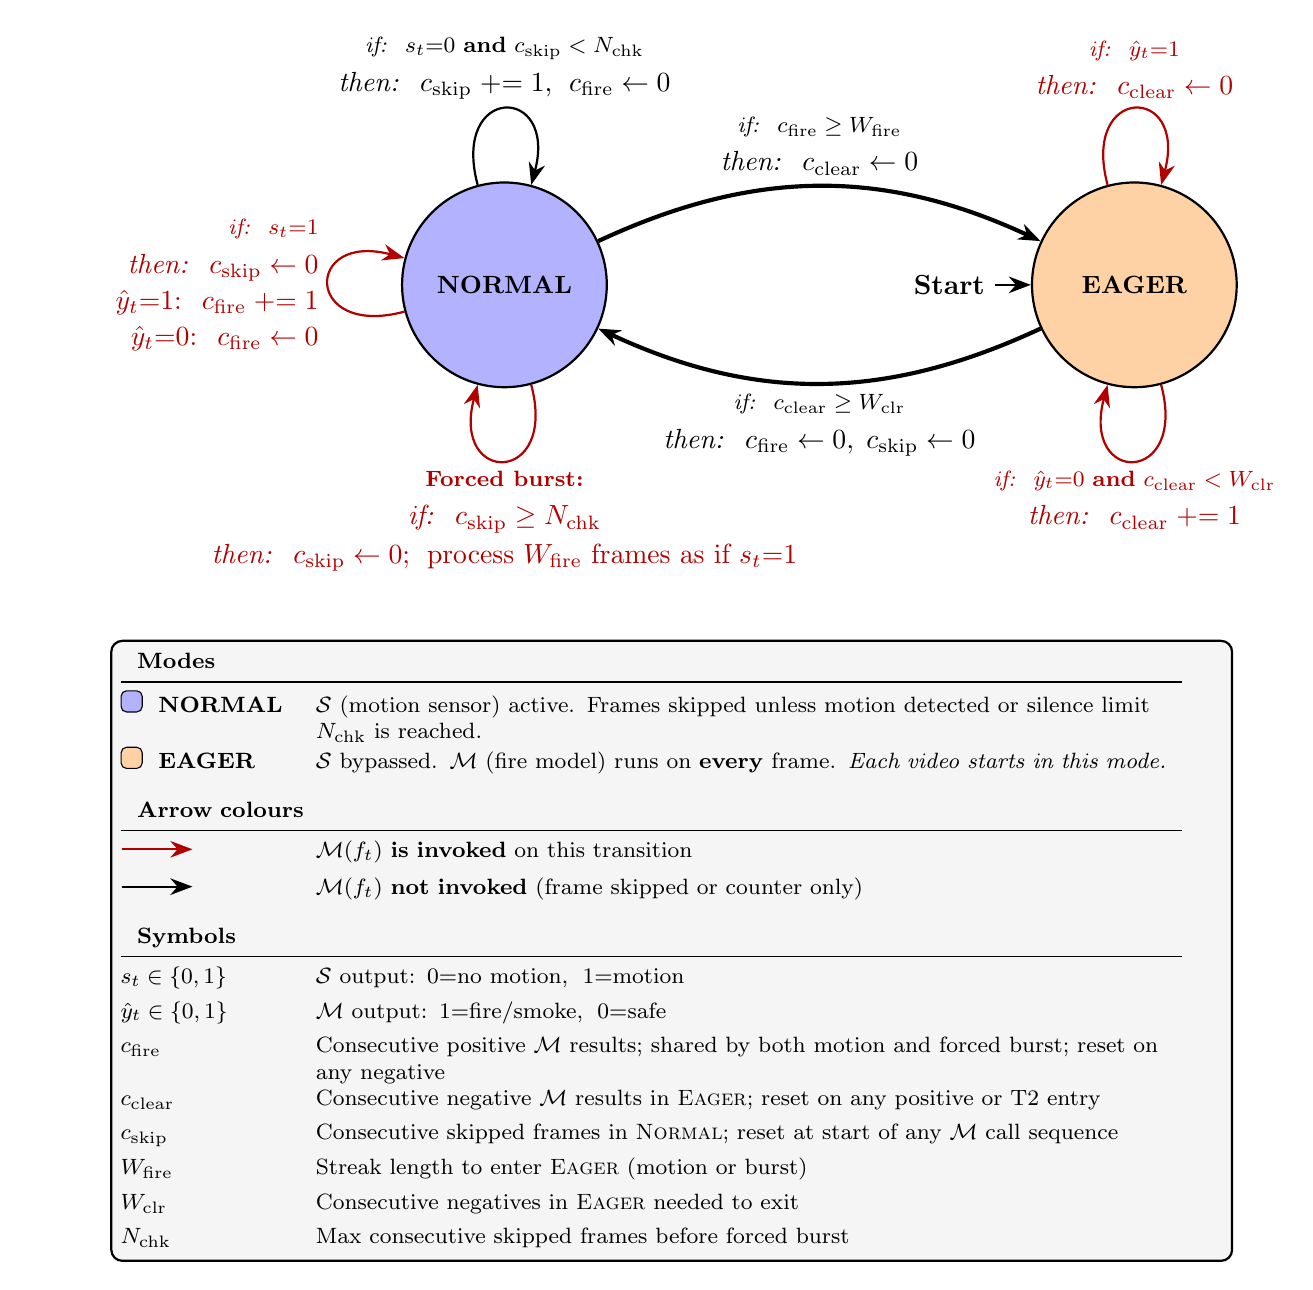
\begin{tikzpicture}[
        node distance=8cm,
        every state/.style={draw, rounded corners, minimum width=2.6cm,
            minimum height=1.3cm, font=\small\bfseries},
        thick,
        >={Stealth[length=8pt, width=6pt]},
        auto
    ]

    %% ── States ───────────────────────────────────────────────────────
    \node[state, fill=blue!30, align=center] (normal) {NORMAL};
    \node[state, initial, initial where=left,
          initial text={\textbf{Start}},
          fill=orange!35, align=center,
          right of=normal] (eager) {EAGER};

    %% ── T1: EAGER → NORMAL ───────────────────────────────────────────
    \draw[->, line width=1.5pt] (eager) edge[bend left=25]
        node[below, align=center]{%
            \footnotesize
            \textit{if:}\; $c_{\mathrm{clear}} \geq W_{\mathrm{clr}}$\\[2pt]
            \textit{then:}\;
            $c_{\mathrm{fire}} \leftarrow 0,\;
             c_{\mathrm{skip}} \leftarrow 0$}
        (normal);

    %% ── T2: NORMAL → EAGER ───────────────────────────────────────────
    \draw[->, line width=1.5pt] (normal) edge[bend left=25]
        node[above, align=center]{%
            \footnotesize
            \textit{if:}\; $c_{\mathrm{fire}} \geq W_{\mathrm{fire}}$ \\[2pt]
            \textit{then:}\; $c_{\mathrm{clear}} \leftarrow 0$}
        (eager);

    %% ── NORMAL top loop: skip ────────────────────────────────────────
    \draw[->] (normal) edge[loop above, looseness=5]
    node[above, align=center]{%
        \footnotesize
        \textit{if:}\;
        $s_t{=}0$ \textbf{and}
        $c_{\mathrm{skip}} < N_{\mathrm{chk}}$ \\[2pt]
        \textit{then:}\; $c_{\mathrm{skip}} \mathrel{+}= 1$,\;
        $c_{\mathrm{fire}} \leftarrow 0$
        }
    (normal);

    %% ── NORMAL left loop: motion (M invoked) ────────────────────────
    \draw[->, red!70!black] (normal) edge[loop left, looseness=5]
        node[left, align=right]{%
            \footnotesize
            \textit{if:}\; $s_t{=}1$ \\[2pt]
            \textit{then:}\; $c_{\mathrm{skip}} \leftarrow 0$ \\[1pt]
            \phantom{\textit{then:}\;}
                $\hat{y}_t{=}1$:\;
                $c_{\mathrm{fire}} \mathrel{+}= 1$ \\[1pt]
            \phantom{\textit{then:}\;}
                $\hat{y}_t{=}0$:\;
                $c_{\mathrm{fire}} \leftarrow 0$}
        (normal);

    %% ── NORMAL bottom loop: forced burst ────────────────────────────
    \draw[->, red!70!black] (normal) edge[loop below, looseness=5]
        node[below, align=center]{%
            \footnotesize
            \textbf{Forced burst:}\\[2pt]
            \textit{if:}\; $c_{\mathrm{skip}} \geq N_{\mathrm{chk}}$ \\[2pt]
            \textit{then:}\; $c_{\mathrm{skip}} \leftarrow 0$;\;
                process $W_{\mathrm{fire}}$ frames as if $s_t{=}1$}
        (normal);

        %% ── EAGER top loop: positive ─────────────────────────────────────
    \draw[->, red!70!black] (eager) edge[loop above, looseness=5]
        node[above, align=center]{%
            \footnotesize
            \textit{if:}\; $\hat{y}_t{=}1$ \\[2pt]
            \textit{then:}\; $c_{\mathrm{clear}} \leftarrow 0$}
        (eager);

    %% ── EAGER bottom loop: negative ──────────────────────────────────
    \draw[->, red!70!black] (eager) edge[loop below, looseness=5]
        node[below, align=center]{%
            \footnotesize
            \textit{if:}\; $\hat{y}_t{=}0$ \textbf{and}
            $c_{\mathrm{clear}} < W_{\mathrm{clr}}$ \\[2pt]
            \textit{then:}\; $c_{\mathrm{clear}} \mathrel{+}= 1$}
        (eager);

    %% ── Legend ───────────────────────────────────────────────────────
    \node[draw, rounded corners, fill=gray!8,
          below=3.2cm of normal,
          anchor=north west, xshift=-5.0cm,
          text width=14cm, font=\footnotesize] (legend) {%
        \begin{tabular}{@{}lp{11cm}@{}}
            \multicolumn{2}{l}{\textbf{Modes}} \\
            \midrule
            \tikz\draw[fill=blue!30, draw=black, rounded corners=2pt]
                (0,0) rectangle (0.9em, 0.9em);
            ~\textbf{NORMAL}
                & $\mathcal{S}$ (motion sensor) active. Frames skipped
                  unless motion detected or silence limit $N_{\mathrm{chk}}$
                  is reached. \\[4pt]
            \tikz\draw[fill=orange!35, draw=black, rounded corners=2pt]
                (0,0) rectangle (0.9em, 0.9em);
            ~\textbf{EAGER}
                & $\mathcal{S}$ bypassed. $\mathcal{M}$ (fire model)
                  runs on \textbf{every} frame.
                  \textit{Each video starts in this mode.} \\[8pt]
            \multicolumn{2}{l}{\textbf{Arrow colours}} \\
            \midrule
            \tikz\draw[->, red!70!black, thick] (0,0) -- (0.9,0); &
                $\mathcal{M}(f_t)$ \textbf{is invoked} on this transition \\[4pt]
            \tikz\draw[->, black, thick] (0,0) -- (0.9,0); &
                $\mathcal{M}(f_t)$ \textbf{not invoked}
                (frame skipped or counter only) \\[8pt]
            \multicolumn{2}{l}{\textbf{Symbols}} \\
            \midrule
            $s_t \in \{0,1\}$
                & $\mathcal{S}$ output: $0$=no motion,\; $1$=motion \\[3pt]
            $\hat{y}_t \in \{0,1\}$
                & $\mathcal{M}$ output: $1$=fire/smoke,\; $0$=safe \\[3pt]
            $c_{\mathrm{fire}}$
                & Consecutive positive $\mathcal{M}$ results; shared by
                  both motion and forced burst; reset on any negative \\[3pt]
            $c_{\mathrm{clear}}$
                & Consecutive negative $\mathcal{M}$ results in
                  \textsc{Eager}; reset on any positive or T2 entry \\[3pt]
            $c_{\mathrm{skip}}$
                & Consecutive skipped frames in \textsc{Normal};
                  reset at start of any $\mathcal{M}$ call sequence \\[3pt]
            $W_{\mathrm{fire}}$
                & Streak length to enter \textsc{Eager} (motion or burst) \\[3pt]
            $W_{\mathrm{clr}}$
                & Consecutive negatives in \textsc{Eager} needed to exit \\[3pt]
            $N_{\mathrm{chk}}$
                & Max consecutive skipped frames before forced burst \\
        \end{tabular}
    };

\end{tikzpicture}
\end{document}